\باب{دہری منطق اور عددی الیکٹرانکس}

اس باب میں دہری منطق اور اس پر بنیاد عددی الیکٹرانکس پر غور ہو گا۔

\حصہ{دہری منطق}
ایک دہری عدد کے دو ہی ممکنہ قیمتیں ہیں یعنی 0 اور 1۔ان دو قیمتوں سے دو متضاد پہلو ظاہر کئے جا سکتے ہیں مثلا درست اور غلط، بلند اور پست، ہوشیار اور آرام باش ،چالو اور بند وغیرہ۔ اگر بلندی کو 1 سے ظاہر کیا جائے تو پستی 0 سے ظاہر ہو گی۔اس کے برعکس اگر بلندی کو 0 سے ظاہر کیا جائے تو پستی 1 سے ظاہر ہو گی۔ان دو طریقوں میں کسی ایک طریقہ کو دوسرے طریقہ پر کوئی فوقیت حاصل نہیں۔

\حصہ{دہری مواد کے نظامِ نمائندگی}
عددی الیکٹرانکس میں دہری عدد کے دو ممکنہ قیمتوں 0 اور 1 کو عموما دو مختلف برقی دباؤ سے ظاہر کیا جاتا ہے۔ \حاشیہد{برقی دباؤ کی جگہ برقی بہاؤ کا استعمل بھی ممکن ہے} اگر 0 کو کم برقی دباؤ اور 1  کو زیادہ برقی دباؤ سے ظاہر کیا جائے تو اسے  دہری مواد کی مثبت نظامِ نمائندگی \حاشیہب{positive representation} کہتے ہیں اور اگر اس کے برعکس 0 کو زیادہ برقی دباؤ اور 1 کو کم برقی دباؤ سے ظاہر کیا جائے تو اسے دہری مواد کی منفی نظامِ نمائندگی \حاشیہب{negative representation} کہتے ہیں۔الیکٹرانکس میں زیادہ برقی دباؤ عموما مثبت پانچ وولٹ لی جاتی ہے جبکہ کم برقی دباؤ صفر وولٹ لی جاتی ہے۔جدید الیکٹرانکس میں زیادہ برقی دباؤ کی مقدار کم کر کے مثبت تین وولٹ کے قریب کر دی گئی ہے۔مساوات \حوالہ{مساوات۔مثبت۔نظام۔نمائندگی} میں دہری عدد 0 کو کم برقی دباؤ یعنی صفر وولٹ اور دہری عدد 1 کو زیادہ برقی دباؤ یعنی مثبت پانچ وولٹ سے ظاہر کیا گیا ہے۔اس کتاب میں صفر وولٹ اور مثبت پانچ وولٹ استعمال کرتے ہوئے دہری مواد کی مثبت نظامِ نمائندگی استعمال کی جائے گی۔موجودہ الیکٹرانکس میں بیشتر طور یہی نظام استعمال ہوتا ہے۔

\begin{align} \label{مساوات۔مثبت۔نظام۔نمائندگی}
0 &= 0 v   \notag \\
1 & = +5 v
\end{align}

اگر کسی پنیہ پر دہری مواد 1 موجود ہو تو یہاں مثبت پانچ برقی دباؤ پائی جائے گی۔اس صورت میں الیکٹرانکس انجنئیر کہیں گے کہ یہ پنیہ بلند حالت \حاشیہب{high state} میں ہے یا کہ یہ پنیہ بلند \حاشیہب{high} ہے۔ اسی طرح اگر ایک پنیہ پر دہری مواد 0 ہو تو یہاں صفر وولٹ کی برقی دباؤ پائی جائے گی۔اس صورت میں الیکٹرانکس انجنئیر کہیں گے کہ یہ پنیہ پست حالت  \حاشیہب{low state} میں ہے یا کہ یہ پنیہ پست \حاشیہب{low} ہے۔اسی طرح کسی پنیہ پر مثبت پانچ وولٹ برقی دباؤ لاگو کرنے کو الیکٹرانکس انجنئیر  اس پنیہ کو بلند کرنا کہتے ہیں اور اس پر صفر وولٹ برقی دباؤ لاگو کرنے کو پنیہ کو پست کرنا کہتے ہیں۔لہٰذا اگر پنیہ بلند ہے تو اس پر دہری مواد 1 ہے اور اگر یہ پست ہے تو اس پر دہری مواد 0 ہے۔

بلند اور پست کی جگہ درست اور غلط کے الفاظ بھی رائج ہیں۔ اس صورت میں دہری مواد 1 کو درست حالت \حاشیہب{true state} یا درست \حاشیہب{true} کہتے ہیں جبکہ دہری مواد 0 کو غلط حالت \حاشیہب{false state} یا غلط \حاشیہب{false} کہتے ہیں۔


\حصہ{درآمدات اور برآمدات}
شکل \حوالہ{شکل۔درآمدی۔برآمدی۔پنیاں} میں الیکٹرانکس کا آلہ دکھایا گیا ہے۔اس کے بائیں جانب دو پنیہ اور دائیں جانب ایک پنیہ ہیں۔بائیں جانب دو پنیہ کے ذریعہ اس آلہ کو دہری مواد فراہم کی جاتی ہے لہٰذا  انہیں درآمدی پنیاں \حاشیہب{input pins} یا درآمدات \حاشیہب{inputs} کہتے ہیں۔دائیں جانب کے پنیہ کے ذریعہ یہ آلہ دہری مواد خارج کرتا ہے لہٰذا اسے برآمدی پنیہ \حاشیہب{output pin} یا برآمد \حاشیہب{output} کہتے ہیں۔الیکٹرانکس میں اسی طرز کو استعمال کرتے ہوئے کسی بھی آلہ کی درآمدی پنیہ یعنی درآمدات کو شکل کے بائیں جانب اور اس کی برآمدی پنیہ یعنی برآمدات کو شکل کے دائیں جانب دکھایا جاتا ہے۔


\begin{figure}[th]
 \begin{center}
  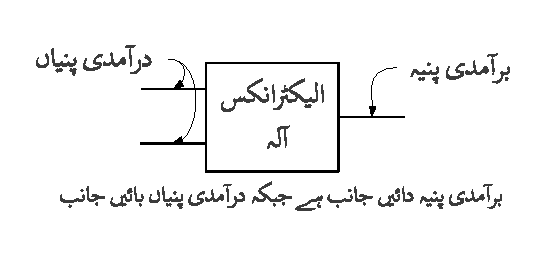
\includegraphics[]{درآمدی۔برآمدی۔پنیاں}
 \end{center}
\caption{درآمدی اور برآمدی پنیاں}
\label{شکل۔درآمدی۔برآمدی۔پنیاں}
\end{figure}


اگر اس شکل میں کسی درآمدی پنیہ پر صفر وولٹ کا برقی دباؤ لاگو کیا جائے تو یہ آلہ اس کو دہری مواد 0 تصور کرے گا اور اگر  اس پر مثبت پانچ وولٹ کا برقی دباؤ لاگو کیا جائے تو یہ آلہ اس کو دہری مواد 1 تصور کرے گا۔اسی طرح اگر یہ آلہ دہری مواد 1 خارج کرنا چاہے تو یہ اپنی برآمدی پنیہ پر مثبت پانچ وولٹ کا برقی دباؤ لاگو کر لے گا اور اگر یہ دہری مواد 0 خارج کرنا چاہے تو یہ اپنی برآمدی پنیہ پر صفر وولٹ کا برقی دباؤ لاگو کر لے گا۔

اس حصہ میں عددی الیکٹرانکس کے چند مخصوص آلات پر غور کیا جائے گا۔یہ آلات عددی الیکٹرانکس میں قلیدی کردار ادا کرتے ہیں۔

\حصہ{اور گیٹ}
شکل \حوالہ{شکل۔دو۔درآمدی۔اور۔گیٹ} میں دو درآمدی اور گیٹ \حاشیہب{AND gate} کی علامت دکھائی گئی ہے۔اس آلہ کی خصوصیت یہ ہے کہ اگر اس کے دونوں درآمدی پنیوں پر دہری مواد 1 فراہم کی جائے تو یہ اپنی برآمدی پنیہ پر 1 خرج کرتا ہے۔یعنی اگر اس کے دونوں درآمدی پنیہ بلند کر دئے جائیں تو اس کا برآمدی پنیہ بلند صورت اختیار کر لیگا۔اگر اس آلہ کے کسی ایک درآمدی پنیہ کو بھی پست کیا جائے تو یہ اپنی برآمدی پنیہ کو پست مقام پر لی جاتا ہے۔

\begin{figure}[th]
 \begin{center}
  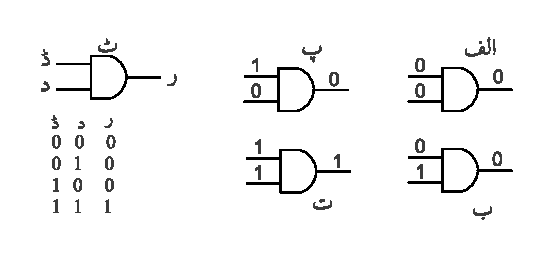
\includegraphics[]{دو۔درآمدی۔اور۔گیٹ}
 \end{center}
\caption{دو درآمدی اور گیٹ}
\label{شکل۔دو۔درآمدی۔اور۔گیٹ}
\end{figure}

شکل کے حصہ الف میں دونوں درآمدی پنیوں پر دہری مواد 0 مہیا کیا گیا ہے۔درآمدی پنیوں پر 0 لکھ کر اس بات کو دکھایا گیا ہے۔اس صورت میں آلہ اپنی برآمدی پنیہ پر 0 ہی خارج کرتا ہے۔برآمدی پنیہ پر 0 لکھ کر ایسا ہوتا دکھایا گیا ہے۔شکل کے حصہ ب اور حصہ پ میں ایک درآمدی پنیہ پر دہری مواد 0 اور دوسری پر دہری مواد  1 مہیا کی گئی ہے۔ ان دونوں صورتوں میں بھی آلہ کی برآمدی پنیہ پر دہری مواد 0 ہی پائی جاتی ہے۔شکل کے حصہ ت میں آلہ کے دونوں درآمدی پنیہ بلند کئے گئے ہیں۔ اس صوارت میں آلہ اپنی برآمدی پنیہ بلند کئے ہوئے ہے۔

شکل کے حصہ ٹ میں آلہ کے دو درآمدی پنیوں کو د اور ڈ نام دئے گئے ہیں جبکہ اس کی برآمدی پنیہ کو ر کا نام دیا گیا ہے۔یوں شکل کے حصہ الف، ب، پ اور ت کے نتائج یکجا کر کے ایک فہرست کی صورت میں لکھے جا سکتے ہیں۔ایسا ہی شکل میں کیا گیا ہے۔یہ فہرست مساوات \حوالہ{مساوات۔اور۔گیٹ} میں دی گئی ہے۔

\begin{align}  \label{مساوات۔اور۔گیٹ}
00 & =0 \notag \\
01 & =0 \notag \\
10 &=0 \notag \\
11 &=1  
\end{align}

درآمدی پنیوں پر دہری مواد کو درآمدات کہتے ہیں اور برآمدی پنیہ پر دہری مواد کو برآمد یا برآمدات کہتے ہیں۔شکل میں د اور ڈ درآمدات اس مساوات میں قریب قریب لکھے گئے ہیں۔مساوات کی دائیں جانب آلہ کی برآمد ر لکھی گئی ہے۔

اس قسم کے آلہ کے دو سے زیادہ درآمدات ہو سکتے ہیں۔ شکل \حوالہ{شکل۔تین۔درآمدی۔اور۔گیٹ} میں تین درآمدی اور گیٹ دکھایا گیا ہے۔د، ڈ اور ذ اس کے درآمدات ہیں جبکہ ر اس کی برآمد ہے۔اس آلہ کی برآمد صرف اس صورت 1 ہو گی جب اِس کے تمام درآمدات 1 ہوں۔شکل میں ایک فہرست یہی واضح کرتی ہے۔

آلہ کے اس خصوصیت کو یوں بھی بیان کیا جا سکتا ہے کہ اس کی برآمد صرف اس صورت 1 ہو گی جب اس کے درآمدات د اور ڈ اور ذ تمام 1 ہوں۔اسی جملے سے اس آلہ کا نام آلہِ  اور \حاشیہب{AND device} نکلا ہے۔



\begin{figure}[th]
 \begin{center}
  \includegraphics[]{تین۔درآمدی۔اور۔گیٹ}
 \end{center}
\caption{تین درآمدی اور گیٹ}
\label{شکل۔تین۔درآمدی۔اور۔گیٹ}
\end{figure}

\حصہ{فہرستِ درستگی}

کسی بھی آلہ کا مطالعہ کرتے وقت اس کے درآمدات کے تمام ممکنہ ترتیب ایک فہرست میں لکھ کر ان کے سامنے اسی ترتیب سے آلہ کے برآمدات لکھے جاتے ہیں۔درآمدات کی ہر ممکنہ ترتیب لکھنے کا آسان طریقہ یہ ہے کہ انہیں دہری گنتی کی شکل میں لکھا جائے۔یوں تین درآمدی آلہ کے لئے تین اعداد پر مشتمل دہری گنتی لکھی جائے گی۔مساوات \حوالہ{مساوات۔تین۔دہری۔اعداد۔کی۔گنتی} میں تین دہری اعداد پر مشتمل گنتی لکھ کر ان کے سامنے مساوات کے نشان لکھے گئے ہیں۔اوپر شکل میں ہر درآمدی ترتیب کے سامنے آلہ کی برآمد لکھی گئی ہے۔

شکل میں دکھائے فہرست میں دہری عدد 1 کو درست اور دہری عدد 0 کو غلط تصور کرتے ہوئے اس فہرست کو فہرستِ درستگی \حاشیہب{truth table} کہا جاتا ہے۔ 

\begin{align}  \label{مساوات۔تین۔دہری۔اعداد۔کی۔گنتی}
000=  \notag \\
001=  \notag \\
010=  \notag \\
011=  \notag \\
100=  \notag \\
101=  \notag \\
110=  \notag \\
111= 
\end{align}

شکل \حوالہ{شکل۔دو۔درآمدی۔اور۔گیٹ} کی طرف دوبارہ توجہ دیں۔اگر اس کی درآمد ڈ کو 0 رکھا جائے جبکہ درآمد د 0 اور 1 دونوں صورتیں اختیار کر سکے تو اس کی برآمد 0 ہی رہتی ہے۔البتہ اگر درآمد ڈ کو 1 رکھا جائے اور درآمد د 0 اور 1 صورت اختیا کرے تب برآمد وہی صورت اختیار کرتا ہے جو درآمد د کی ہو۔اس سے واضح ہے کہ اگر درآمد ڈ کو 0 رکھا جائے تو درآمد د پر دی گئی دہری مواد آلہ سے گزر کر اس کی برآمد نہیں بن جاتی جبکہ اگر درآمد ڈ کو 1 رکھا جائے تو اس آلہ کی برآمد وہی ہوتی ہے جو اس کی درآمد د ہو۔یہ آلہ ایک دروازہ کی حیصیت سے کام کر رہا ہے جس کو بند اور کھول کر کے دہری مواد د کو آلہ سے گزرنے سے روکھا جا سکتا ہے یا پھر اسے گزرنے دیا جا سکتا ہے۔اس خوبی کی وجہ سے اس آلہ کو گیٹ کہا جاتا ہے اور یوں اسے دو درآمدی اور گیٹ کہتے ہیں۔

دو درآمدی اور گیٹ کے کسی ایک درآمدی پنیہ کے ذریعہ اس گیٹ کو بند یا کھولا جا سکتا ہے۔اسی طرح دو سے زیادہ درآمدی اور گیٹ کو بھی کسی ایک یا ایک سے زیادہ درآمدات کی مدد سے بند یا کھولا جا سکتا ہے۔جس درآمدی پنیہ سے گیت قابو کیا جاتا ہو اس کو گیٹ کی قابو پنیہ \حاشیہب{control pin} کہتے ہیں اور اس قابو کرنے والے درآمد کو قابو کی درآمد \حاشیہب{control input} کہتے ہیں۔شکل \حوالہ{شکل۔ایک۔عدد۔کا۔گیٹ} میں دو درآمدات کے اور گیٹ کو اس طرح استعمال ہوتے دکھایا گیا ہے۔


\begin{figure}[th]
 \begin{center}
  \includegraphics[]{ایک۔عدد۔کا۔گیٹ}
 \end{center}
\caption{اور۔گیٹ}
\label{شکل۔ایک۔عدد۔کا۔گیٹ}
\end{figure}
\حصہ{اور گیٹ کی ضرب کرنے کی صلاحیت}

شکل \حوالہ{شکل۔اور۔گیٹ۔سے۔ضرب} میں دو درآمدی اور گیٹ دکھایا گیا ہے جس کے درآمدات کو a اور b کا نام دیا گیا ہے۔ہمیں معلوم ہے کہ 


\begin{align*}
0 \times 0 &=0 \\
0 \times 1 &=0 \\
1 \times 0 &=0 \\
1 \times 1 &=1
\end{align*}


شکل میں اس طرح a اور b کے چاروں ممکنہ حاصلِ ضرب دکھائے گئے ہیں۔اسی شکل میں دو درآمدات اور گیٹ کی فہرستِ درستگی بھی دکھائی گئی ہے۔ان دو نتائج کو دیکھنے سے معلوم ہوتا ہے کہ یہ بالکل یکساں ہیں۔اگر دو سے زیادہ درآمدات کی اور گیٹ کا مطالعہ کیا جائے تو یہی نتیجہ نکلتا ہے۔اس سے معلوم ہوا کہ اور گیٹ دہری اعداد کو ضرب کرتا ہے۔شکل میں اور گیٹ پر ضرب کی نشان اسی بات کو ظاہر کرتی ہے۔یوں دو درآمدات کی اور گیٹ کے لئے ہم  مساوات \حوالہ{مساوات۔اور۔گیٹ۔سے۔دہری۔ضرب} لکھ سکتے ہیں۔ضرب کو صلیب کی نشان یا پھر نکتہ سے ظاہر کیا جاتا ہے۔مساوات میں دونوں طریقے دکھلائے گئے ہیں۔

\begin{align}   \label{مساوات۔اور۔گیٹ۔سے۔دہری۔ضرب}
c &=a \times b \\
c &=a \cdot b
\end{align}


\begin{figure}[th] 
 \begin{center}
  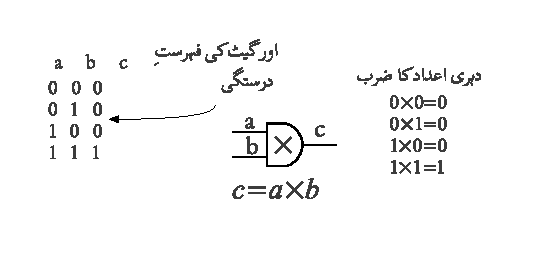
\includegraphics[]{اور۔گیٹ۔سے۔ضرب}
 \end{center}
\caption{اور گیٹ سے ضرب حاصل کرنا}
\label{شکل۔اور۔گیٹ۔سے۔ضرب}
\end{figure}


\حصہ{یا گیٹ}
دو درآمدی یا گیٹ \حاشیہب{OR gate} اور تین درآمدی یا گیٹ کی علامتیں شکل \حوالہ{شکل۔یا۔گیٹ۔کی۔علامت} میں دکھائی گئی ہیں۔تین درآمدی یا گیٹ کی خصوصیات یوں بیان کی جا سکتی ہے کہ اس کی برآمد اُس صورت 1 ہوتی ہے جب اس کی پہلی یا دوسری یا تیسری درآمد 1 ہو۔اسی جملے کی وجہ سے اس آلہ کا نام یا گیٹ ہے۔

\begin{figure}[th]
 \begin{center}
  \includegraphics[]{یا۔گیٹ۔کی۔علامت}
 \end{center}
\caption{یا گیٹ کی علامتیں اور ان کی فہرستِ درستگی}
\label{شکل۔یا۔گیٹ۔کی۔علامت}
\end{figure}

یا گیٹ کی فہرستِ درستگی کو اور گیٹ کی فہرستِ درستگی کے ساتھ دیکھیں۔ یا گیٹ کی برآمد تمام ممکنہ درآمدات کی ترتیبوں میں صرف ایک ترتیب کے لئے درست ہے جبکہ اور گیٹ کی برآمد تمام ممکنہ درآمدات کی ترتیبوں میں صرف ایک ترتیب کے لئے غلط ہے۔

مساوات \حوالہ{مساوات۔دو۔دہری۔اعداد۔کا۔مجموعہ} میں ایک ہندسے کے دو دہری اعداد کے ممکنہ مجموعے دکھائے گئے ہیں۔یہ دو درآمدی یا گیٹ کی فہرستِ درستگی کے ساتھ بہت مشابہت رکھتا ہے۔ان دونوں میں صرف ایک جمع ایک کرتے وقت فرق ہے۔اسی مشابہت کی وجہ سے یا گیٹ کو جمع کی علامت سے ظاہر کیا جاتا ہے۔یہ دھان رکھنا ضروری ہے کہ یا گیٹ استعمال کرتے وقت جمع کا مطلب ہرگز الجبرا کے جمع کا نشان نہیں۔

\begin{align} \label{مساوات۔دو۔دہری۔اعداد۔کا۔مجموعہ}
0+0 &=0 \notag \\
0+1 &=1 \notag \\
1+0 &=1 \notag \\
1+1 &=2
\end{align}

مساوات \حوالہ{مساوات۔یا۔گیٹ۔سے۔حاصل۔جمع} میں دو درآمدی یا گیٹ کی فہرستِ درستگی کو + کا نشان استعمال کرتے لکھا گیا۔
شکل  \حوالہ{شکل۔یا۔گیٹ۔سے۔حاصل۔جمع} میں دو اور تین درآمدی یا گیٹ اور ان کی فہرستِ درستگی + کے نشان استعمال کرتے  دکھائے گئے ہیں۔


\begin{align} \label{مساوات۔یا۔گیٹ۔سے۔حاصل۔جمع}
0+0 &=0 \notag \\
0+1 &=1 \notag \\
1+0 &=1 \notag \\
1+1 &=1
\end{align}

\begin{figure}[th]
 \begin{center}
  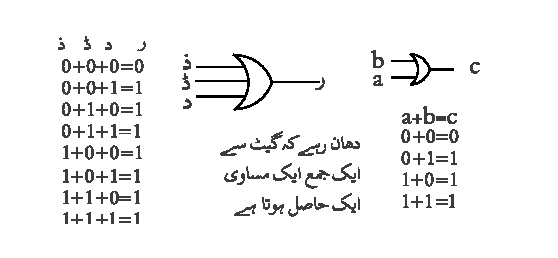
\includegraphics[]{یا۔گیٹ۔سے۔حاصل۔جمع}
 \end{center}
\caption{یا گیٹ سے حاصل جمع}
\label{شکل۔یا۔گیٹ۔سے۔حاصل۔جمع}
\end{figure}

\جزحصہ{بطورِ گیٹ}
دو درآمدی یا گیٹ کی اگر ایک درآمدی پنیہ کو قابو کی پنیہ  اور دوسری درآمدی پنیہ کو اس کی داخل مواد کی پنیہ تصور کرتے ہوئے جب تک قابو کی پنیہ بلند رہے اس وقت تک مواد کی پنیہ کو بلند یا پست کرنے سے آلہ کی برآمد پر کوئی اثر نہیں پڑتا اور یہ بتدریج بلند رہتی ہے۔البتہ اگر اس کی قابو کی پنیہ کو پست کیا جائے تب آلہ کی برآمد وہی ہوتی ہے جو اس کے مواد کی پنیہ پر داخل ہو۔یہ شکل \حوالہ{شکل۔یا۔بطور۔ایک۔عدد۔کا۔گیٹ} میں دکھایا گیا ہے۔
 


\begin{figure}[th]
 \begin{center}
  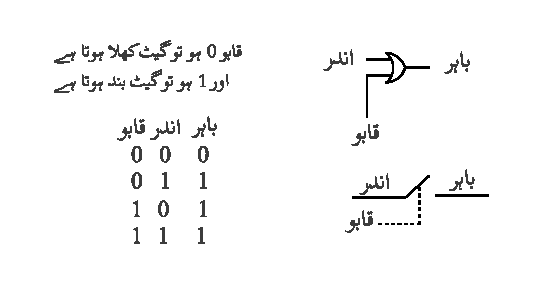
\includegraphics[]{یا۔بطور۔ایک۔عدد۔کا۔گیٹ}
 \end{center}
\caption{یا بطور۔ایک۔عدد۔کا۔گیٹ}
\label{شکل۔یا۔بطور۔ایک۔عدد۔کا۔گیٹ}
\end{figure}

\حصہ{نفی گیٹ}
نفی گیٹ \حاشیہب{NOT gate} کی ایک درآمد اور ایک برآمد ہوتی ہے۔اس گیٹ کی خصوصیت یہ ہے کہ اس کی برآمد ہر وقت اس کی درآمد کی الٹ ہوتی ہے یعنی اگر اس کی درآمد 0 ہو تو یہ 1 برآمد کرتا ہے اور اگر اس کی درآمد 1 ہو تب یہ 0 برآمد کرتا ہے۔شکل \حوالہ{شکل۔نفی۔گیٹ} میں نفی گیٹ کی علامت اور اس کی فہرستِ درستگی دکھائی گئی ہے۔نفی کے عمل کو علامت کے اوپر لکیر سے ظاہر کیا جاتا ہے۔

\begin{figure}[th]
 \begin{center}
  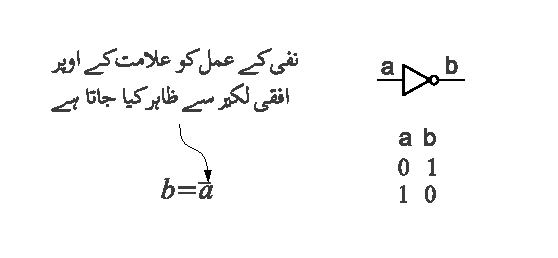
\includegraphics[]{نفی۔گیٹ}
 \end{center}
\caption{نفی۔گیٹ}
\label{شکل۔نفی۔گیٹ}
\end{figure}

\حصہ{نفی یا گیٹ}
جب یا گیٹ کے ساتھ نفی گیٹ شکل \حوالہ{شکل۔نفی۔یا۔گیٹ۔کی۔فہرست۔درستگی} کی طرح جوڑا جائے تو اسے نفی یا گیٹ کہتے ہیں۔نفی یا گیٹ کی علامت اور اس کی فہرستِ درستگی اسی شکل میں دی گئی ہے۔

\begin{figure}[th]
 \begin{center}
  \includegraphics[]{نفی۔یا۔گیٹ۔کی۔فہرست۔درستگی}
 \end{center}
\caption{نفی۔یا۔گیٹ}
\label{شکل۔نفی۔یا۔گیٹ۔کی۔فہرست۔درستگی}
\end{figure}
 
\حصہ{نفی اور گیٹ}
جب اور گیٹ کے ساتھ نفی گیٹ شکل \حوالہ{شکل۔نفی۔اور۔گیٹ۔کی۔فہرست۔درستگی} کی طرح جوڑا جائے تو اسے نفی اور گیٹ کہتے ہیں۔نفی اور گیٹ کی علامت اور اس کی فہرستِ درستگی اسی شکل میں دی گئی ہے۔


\begin{figure}[th]
 \begin{center}
  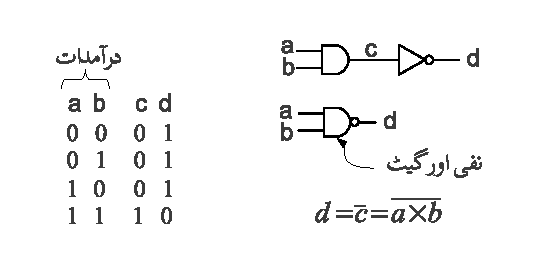
\includegraphics[]{نفی۔اور۔گیٹ۔کی۔فہرست۔درستگی}
 \end{center}
\caption{نفی۔اور۔گیٹ}
\label{شکل۔نفی۔اور۔گیٹ۔کی۔فہرست۔درستگی}
\end{figure}

\حصہ{بلا شرکت یا گیٹ}
بلا شرکت یا گیٹ کی برآمد اس وقت 1 ہوتی ہے جب اس کے درآمدات میں جفت مرتبہ 1 ہو۔اس گیٹ کے ساتھ نفی گیٹ جوڑ کر نفی بلاشرکت یا گیٹ بنایا جاتا ہے۔شکل میں یہ دونوں دکھائے گئے ہیں۔بلاشرکت یا گیٹ کی فہرستِ درستگی کو الجبرائی شکل میں یوں لکھا جاتا ہے۔
\begin{align*}
c=a+b
\end{align*}

\begin{figure}[th]
 \begin{center}
  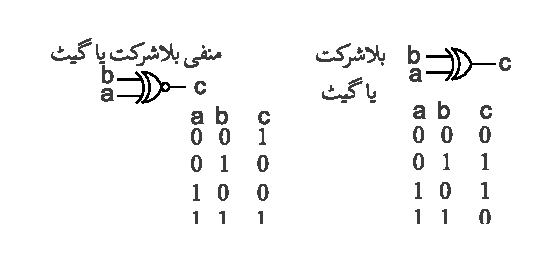
\includegraphics[]{بلاشرکت۔یا۔گیٹ}
 \end{center}
\caption{بلا شرکت یا گیٹ}
\label{شکل۔بلاشرکت۔یا۔گیٹ}
\end{figure}

\حصہ{پلٹ}
شکل \حوالہ{شکل۔نفی۔اور۔گیٹ۔پر۔بنیاد۔پلٹ} میں دو درآمدی نفی اور گیٹ آپس میں ایک مخصوص طریقہ سے جڑے ہیں۔اس برقی دور کے درآمدات کو ہوشیار \حاشیہب{set} اور آرام باش \حاشیہب{reset} کہا گیا ہے جنہیں s اور r سے ظاہر کیا گیا ہے۔اس دور کے برآمدات کو Q اور Q کہا گیا ہے۔

\begin{figure}[th]
 \begin{center}
  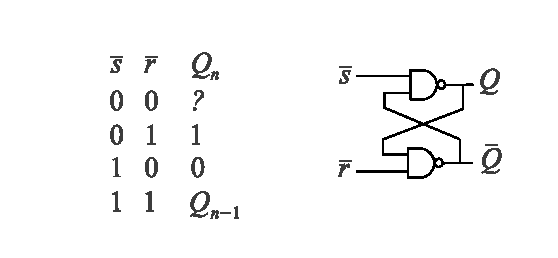
\includegraphics[]{نفی۔اور۔گیٹ۔پر۔بنیاد۔پلٹ}
 \end{center}
\caption{نفی۔اور۔گیٹ۔پر۔بنیاد۔پلٹ}
\label{شکل۔نفی۔اور۔گیٹ۔پر۔بنیاد۔پلٹ}
\end{figure}

اس دور کو استعمال کرتے وقت اس کے دونوں درآمدات بیکوقت پست نہیں کئے جاتے۔شکل میں اس دور کی فہرستِ درستگی بھی دی گئی ہے۔اگر Q بلند ہو تو اس دور کو ہوشیار سمجھا جاتا ہے اور اگر یہ پست ہو تو اسے آرام باش حال میں سمجھا جاتا ہے۔اسی سے اس دور کا نام ہوشیار-آرام باش پلٹ نکلا ہے۔

اگر s پست کیا جائے تو Q بلند ہوتا ہے یعنی دور ہوشیار ہو جاتا ہے جبکہ اگر r پست کیا جائے تو Q پست ہوتا ہے یعنی دور آرام باش حال اختیار کرتا ہے۔اسی سے اس کے دو درآمدات کو ہوشیار اور آرام باش درآمدات کا نام دیا گیا ہے۔اگر دونوں درآمدات بلند رہیں تو دور اپنی حالت برقرار رکھتا ہے۔

